\section{Data acquisition}
\label{sec:data_acquisition}

The second phase of the pipeline is data acquisition. After REPLACE_WE have set up the camera according to the session parameters REPLACE_WE can start recording. REPLACE_WE set a timer for $30s$ and record the RGB and Depth streams from the camera. REPLACE_WE also record the camera intrinsics, which REPLACE_WE will use to recreate the point cloud at a later stage. REPLACE_WE record the data in a folder structure that is defined by the session parameters.

\subsection{Data format}

An important part of data acquisition is the description of the way the data is stored in the file system. This is essential for any future use of the data and therefore REPLACE_WE need to make sure that the data is stored in a way that is easy to understand and easy to use. REPLACE_WE store in general two to five files per session depending on the camera configuration. 

\subsubsection{Session Metadata}

Every session contains a "\texttt{SESSION\_NAME.json}" file that contains the session parameters and camera metadata. The session name is automatically generated based on the starting time of the session, this way REPLACE_WE can make sure that the session name is unique every time and REPLACE_WE can also have an idea of which recording is the most recent without looking at the contents of the file.

\paragraph{Camera metadata}

The camera metadata contains the camera intrinsics, which REPLACE_WE will use to recreate the point cloud at a later stage. The camera intrinsics are the field of view of the depth camera in the horizontal and vertical direction, and the principal point in the horizontal and vertical direction. The field of view is the angle between the optical axis and the image plane. The principal point is the point in the image where the optical axis of the camera intersects the image plane. The principal point and the field of view are explained in Figure \ref{fig:pinhole_camera_model}.

\begin{figure}[ht]
  \centering
  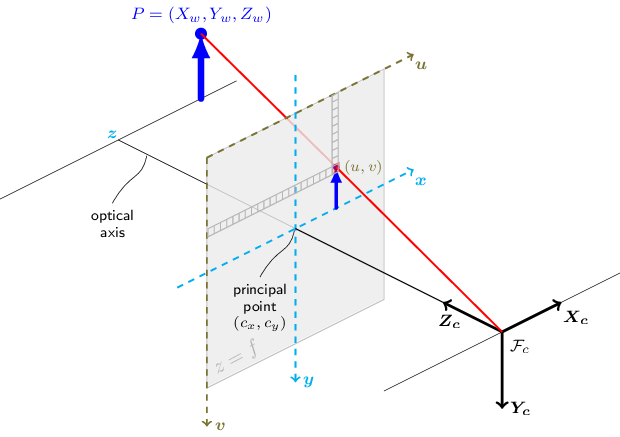
\includegraphics[width=.9\textwidth]{figures/CameraCalibration/pinhole_camera_model.png}
  \caption[Pinhole camera model]{The pinhole camera model that shows the principal point. The principal point is the point where the optical axis intersects the image plane. The field of view is the angle between the optical axis and the image plane.}
  \label{fig:pinhole_camera_model}
\end{figure}

\paragraph{Camera orientation}

Additionally, to the camera intrinsics REPLACE_WE store the relative rotation and translation between the cameras if multiple cameras are used. The rotation and translation are stored as Euler angles\footnote{Technically REPLACE_WE are storing the rotation with the Tait–Bryan notation, i.e. x-y-z or yaw-pitch-roll, rather than the classic Euler notation. However, the name Euler angle is more commonly used and understood.} and a vector respectively \cite{euler1776formulae}. The rotation is the rotation of the camera relative to the second camera in the system. The translation is the translation of the camera concerning the second camera in the system.

\paragraph{Session parameters}

The session parameters are the same as the ones defined in the section "Stream pre-processing". The user enters the session parameters before starting the recording. Most of the parameters are boolean values that indicate whether the user is sitting, wearing dark clothing, etc. The height and angle parameters are the height of the camera to the floor and the angle of the camera relative to the orientation of the user as explained in the previous section.

An example of the Session metadata can be seen in Listing \ref{lst:session_metadata}.

\begin{lstlisting}[language=json,
                   firstnumber=1,
                   caption={[Example of session metadata]{Example of the Session metadata with a single Realsense Camera which was recorded for 40 seconds at around 30 frames per second resulting in 1200 frames. Some values have been changed to increase readability.}},
                   label={lst:session_metadata}]
{
  "Cameras" : 
  [
    {
      "Cx" : 314.26,
      "Cy" : 239.46,
      "FileName" : "Session_2023-01-30T09.21.34_Realsense_Camera_0.bag",
      "Fx" : 459.77,
      "Fy" : 459.83,
      "MeterPerUnit" : 0.00025,
      "Name" : "Realsense Camera 0",
      "Type" : "Realsense"
    }
  ],
  "DurationInSec": 40.0,
  "Name": "Session 2023-01-30T09:21:34",
  "RecordedFrames": 1200,
  "Rotation": {
      "Roll": 0.0,
      "Pitch": 0.0,
      "Yaw": 0.0
  },
  "Translation": {
      "X": 0.0,
      "Y": 0.0,
      "Z": 0.0
  },
  "Session Parameters": {
    "Sitting": true,
    "Background close": true,
    "Cramped": false,
    "Dark Clothing": true,
    "Holding Weight": false,
    "Ankle Weight": false,
    "Height": 1.8,
    "Angle": 20.0
  }
}
\end{lstlisting}

\subsubsection{Realsense Cameras}

We record Realsense Cameras using the librealsense SDK provided by Intel. Using the SDK REPLACE_WE have access to the Hight-Level Pipeline API which allows REPLACE_US to stream the camera feed and access the camera intrinsics. This High-Level Pipeline API allows REPLACE_US to record the RGB and Depth streams from the Realsense camera. The SDK automatically synchronises the Depth and RGB stream as well as the motion sensors, which REPLACE_WE do not use since REPLACE_OUR camera is static. The librealsense SDK is available on GitHub\footnote{\url{https://github.com/IntelRealSense/librealsense}}.

The Recordings are stored in a ROS bag file. A ROS bag file is a file format for storing ROS messages. The ROS bag file format is a container format that stores multiple messages in a single file. The ROS bag file format is described in detail in the ROS wiki\footnote{\url{http://wiki.ros.org/Bags}}. The ROS bag file format is a container format that stores multiple messages in a single file. In REPLACE_OUR case, the important messages are the camera intrinsics, which allow REPLACE_US to create a virtual Realsense Camera from the recording, the RGB stream, and the Depth stream. However, other messages are also stored and can be accessed using the ROS Bag API\footnote{\url{http://wiki.ros.org/rosbag/Code\%20API}}.

\subsubsection{Orbbecc Astra Cameras}

To read the depth stream of the Orbbecc Astra camera REPLACE_WE use the OpenNI2 API\footnote{\url{https://structure.io/openni}}. The OpenNI2 API is a cross-platform API that allows REPLACE_US to access the depth stream of the Orbbecc Astra camera. The OpenNI API is no longer being developed by PrimeSense and has been renamed to OpenNI2 to avoid confusion with the OpenNI API. The OpenNI2 API is available on GitHub\footnote{\url{https://github.com/structureio/OpenNI2}}.

Using the OpenNI2 API REPLACE_WE can also record the depth stream to a file. The depth stream is stored as a \texttt{.ONI} file. The \texttt{.ONI} file format is a proprietary format that is not documented. However, the OpenNI2 API provides a \texttt{.ONI} file reader that allows REPLACE_US to access the depth stream.

Sadly, the OpenNI2 API does not provide a way to access the RGB stream. Therefore, REPLACE_WE use the OpenNI2 API to access the depth stream and OpenCV to access the RGB stream. The RGB stream is stored as a \texttt{.AVI} file. The \texttt{.AVI} file format is a container format that stores multiple video streams in a single file. The \texttt{.AVI} file format is described in detail in the Microsoft documentation\footnote{\url{https://docs.microsoft.com/en-us/previous-versions/ms779636(v=vs.85)}}. 

\textit{
  \textbf{ISSUE}: currently the playback of the \texttt{.AVI} file is only possible at a specific framerate, which is set at the beginning of the recording session. This poses a substantial issue regarding synchronisation. Should I write about this? Should I only use depth data? 
}

\subsection{Recording process}

Once the scene is set and the point clouds have been aligned the user can start the recording. Firstly, there are pre-recording settings such as a frame and/or time limit in seconds, which allows accurate time and/or frame constraints to create equal recordings. Secondly, the user can select whether or not to display the point cloud while recording. This allows the user to see the point cloud in real-time and adjust the recording accordingly, however, this leads to a substantially reduced framerate\footnote{From 30 FPS, without point cloud to 15 FPS with pointcloud}. These can be set in the GUI as shown in Figure \ref{fig:recording_gui}. Finally, the user can configure the session parameters described earlier. After the recording has beend started by the user a preconfigured countdown will be started, allowing the user to get into position in time. Once the countdown has finished the recording will start. The recording will stop once the time or frame limit has been reached. The recording will also stop if the user presses the stop button.  

\begin{figure}[ht]
  \centering
  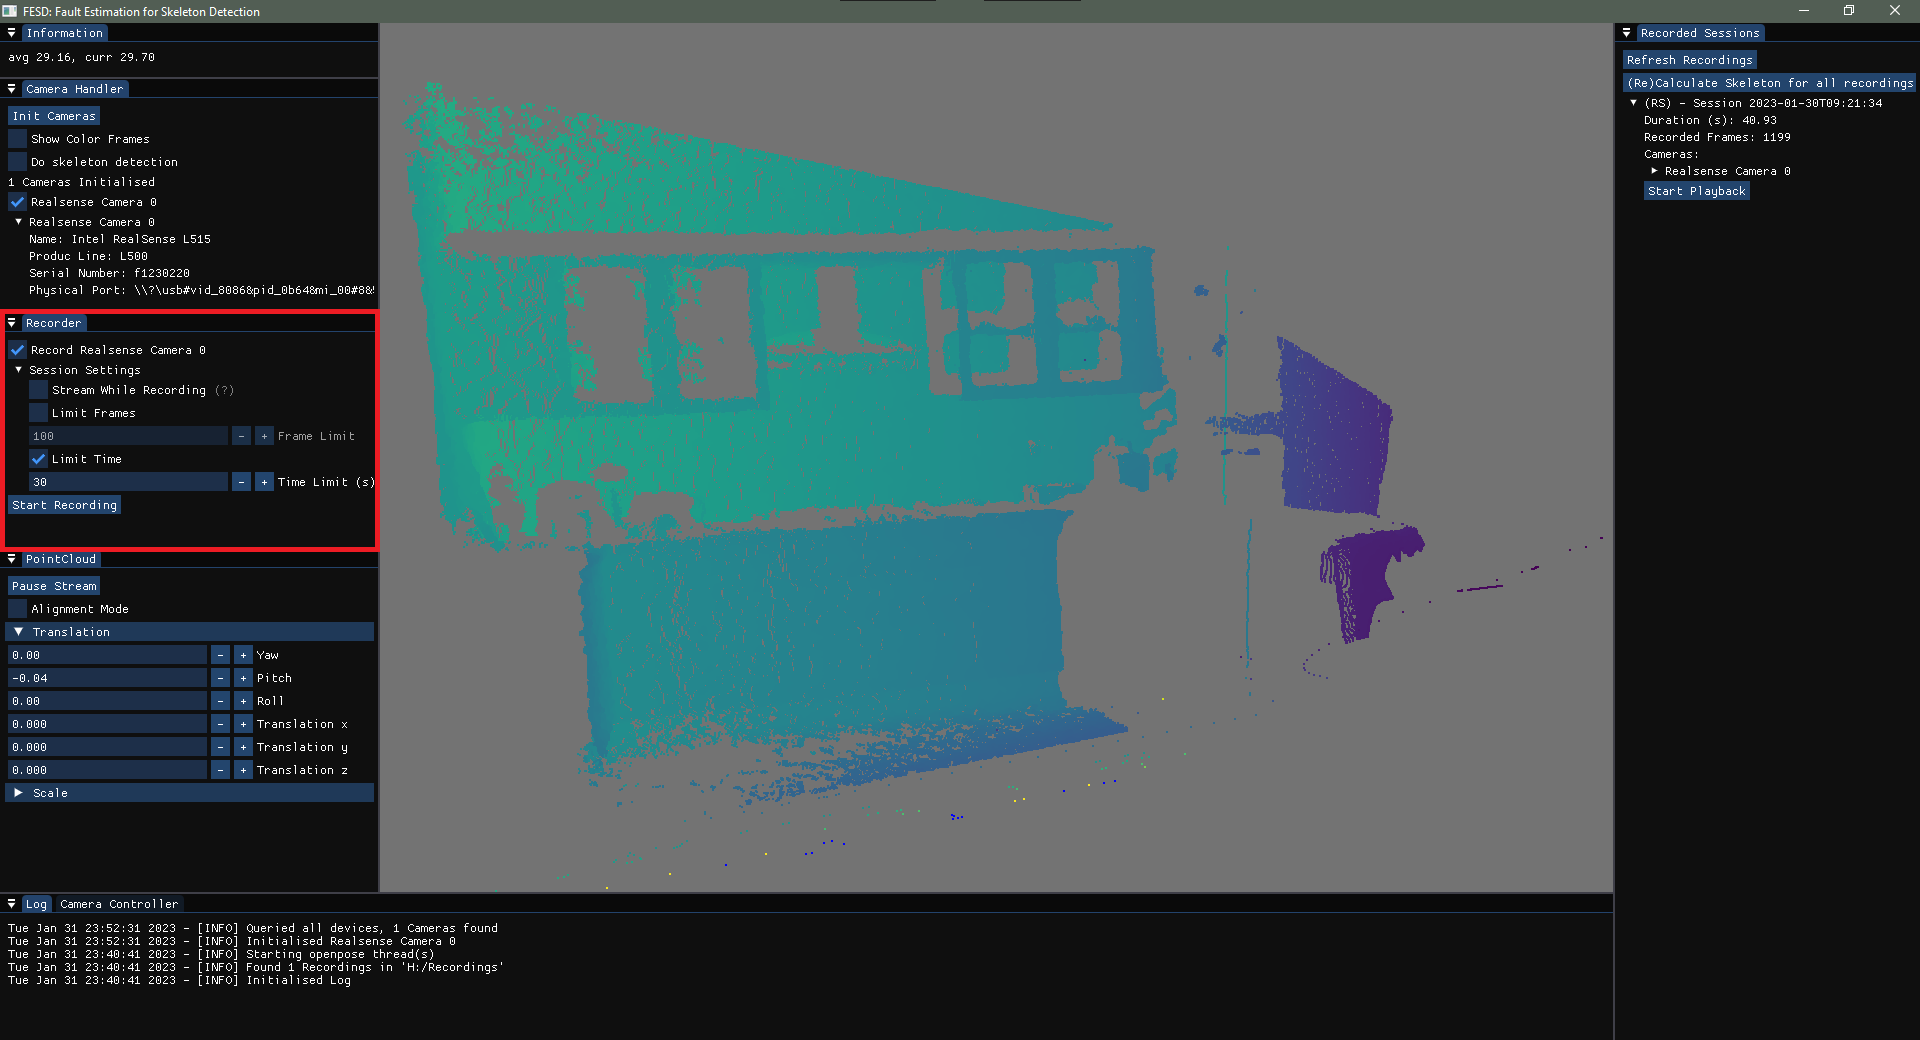
\includegraphics[width=0.8\linewidth]{figures/FESD/recording_gui.png}
  \caption[Recording GUI marked in Red]{Recording GUI marked in Red. The user can set the recording parameters here such as the time and frame limits and whether or not the .}
  \label{fig:recording_gui}
\end{figure}